\documentclass{article}
\usepackage[T1]{fontenc}
\usepackage{lmodern}
\usepackage{graphicx}
\usepackage{amsmath,amssymb}
\usepackage[a4paper,margin=2cm]{geometry}
\usepackage[absolute,overlay]{textpos}
\setlength{\TPHorizModule}{1mm}
\setlength{\TPVertModule}{1mm}
\usepackage[indonesian]{babel}
\usepackage{hyperref}
\setlength{\emergencystretch}{2em}
% unit: Halaman 83

\begin{document}

% === Halaman 83 (python/native) ===

• Column round dan row round dilakukan di dalam sebuah struktur quarter round  

QR(a, b, c, d) yang menerima empat word sebagai masukan dan menghasilkan 

empat word luaran:

      b  b  (a + d) <<<  7;

      c  c   (b + a) <<<  9;

      d  d  (c + b) <<< 13;

      a  a  (d + c) <<< 18;


    <<< k adalah pergeseran bit ke kiri

    sejauh k bit dan bersifat rotasi (siklik)

    + adalah penjumlahan bit dalam mod 232  

83

Quarter Round merupakan inti Salsa20

% deskripsi: gambar native xref 326
\noindent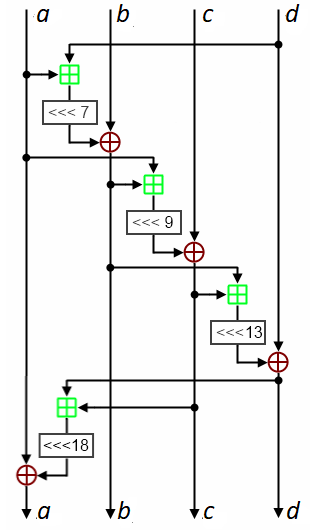
\includegraphics[width=0.85\textwidth]{../../images/python/page_083_img_01.png}

\end{document}
